%% LyX 2.3.4.2 created this file.  For more info, see http://www.lyx.org/.
%% Do not edit unless you really know what you are doing.
\documentclass[10pt,english]{article}
\usepackage[T1]{fontenc}
\usepackage[latin9]{luainputenc}
\usepackage{geometry}
\geometry{verbose,tmargin=3cm,bmargin=3cm,lmargin=2cm,rmargin=2cm,headheight=1cm,headsep=1cm}
\usepackage{fancyhdr}
\pagestyle{fancy}
\usepackage{float}
\usepackage{mathtools}
\usepackage{bm}
\usepackage{amsmath}
\usepackage{amsthm}
\usepackage{graphicx}
\usepackage{esint}

\makeatletter

%%%%%%%%%%%%%%%%%%%%%%%%%%%%%% LyX specific LaTeX commands.
%% Because html converters don't know tabularnewline
\providecommand{\tabularnewline}{\\}

%%%%%%%%%%%%%%%%%%%%%%%%%%%%%% Textclass specific LaTeX commands.
\numberwithin{equation}{section}
\numberwithin{figure}{section}

\@ifundefined{showcaptionsetup}{}{%
 \PassOptionsToPackage{caption=false}{subfig}}
\usepackage{subfig}
\makeatother

\usepackage{babel}
\begin{document}
\title{Fermi Gas}
\date{Jie Ren}
\maketitle

\section{Fourier transformation convention}

We use box normalization so that both momentums and Matsubara frequency
are discrete. We combine the position with time, and similarly momentum
with frequency to form a four-vectors

\begin{eqnarray*}
x & \coloneqq & \left(\bm{x},\tau\right),\\
p & \coloneqq & \left(\bm{p},\omega\right),
\end{eqnarray*}
where Matsubara frequency is:

\[
\omega_{n}=\begin{cases}
2n\pi/\beta & boson\\
\left(2n+1\right)\pi/\beta & fermion
\end{cases}.
\]
For convenience, we define the inner product
\[
p\cdot x\coloneqq\bm{p}\cdot\bm{x}-\omega\tau.
\]
The Fourier transformation of fields is

\begin{eqnarray*}
\psi_{p} & = & \frac{1}{\sqrt{\beta L^{d}}}\int_{0}^{\beta}d\tau\int d^{d}xe^{-ip\cdot x}\psi_{x},\\
\psi_{x} & = & \frac{1}{\sqrt{\beta L^{d}}}\sum_{\omega}\sum_{\bm{p}}e^{+ip\cdot x}\psi_{p}.
\end{eqnarray*}
Strictly speaking, the spatial integral should be written as $\int_{V}d^{d}x$.
While generally, we consider it to be ``semi-infinite'' - while
the integral in done on the infinite space, the system can still have
a macroscopic volume denoted buy $V$.

A slightly different normalization is taken for Fourier transformation
of functions:

\begin{eqnarray*}
f\left(\bm{k}\right) & = & \frac{1}{L^{d}}\int d^{d}xe^{-i\bm{k}\cdot\bm{x}}f\left(\bm{x}\right),\\
f\left(\bm{x}\right) & = & \sum_{k}e^{+i\bm{k}\cdot\bm{x}}f\left(\bm{x}\right).
\end{eqnarray*}
Oftentimes, we are considering a semi-continuous system, where we
can always make the substitution:

\[
\sum_{\bm{k}}\longrightarrow L^{d}\int\frac{d^{d}k}{\left(2\pi\right)^{d}},
\]
and in zero-temperature limit, we can replace frequency sum by integral:
\[
\sum_{l}\longrightarrow\beta\int\frac{d\omega}{2\pi}
\]


\section{Action}

The action of interacting Fermi gas is:

\begin{eqnarray*}
S & = & S_{0}+S_{1},\\
S_{0} & = & \int d^{4}x\sum_{\sigma}\bar{\psi}^{\sigma}\left(x\right)\left(\partial_{\tau}-\frac{\nabla^{2}}{2m}-\mu\right)\psi^{\sigma}\left(x\right),\\
S_{1} & = & \frac{1}{2}\int d^{4}x_{1}\int d^{4}x_{2}\sum_{\sigma,\sigma'}\bar{\psi}^{\sigma}\left(x_{1}\right)\bar{\psi}^{\sigma'}\left(x_{2}\right)V\left(\bm{x}_{1}-\bm{x}_{2}\right)\psi^{\sigma'}\left(x_{2}\right)\psi^{\sigma}\left(x_{1}\right).
\end{eqnarray*}
Where the $V\left(\bm{r}\right)$ is the Coulomb interaction
\[
V\left(\bm{r}\right)=\frac{e^{2}}{r}.
\]
In momentum space:
\[
\psi_{p}^{\sigma}=\sqrt{\frac{T}{L^{3}}}\sum_{p}e^{-ip\cdot x}\psi^{\sigma}\left(x\right).
\]
The action is then

\begin{eqnarray*}
S_{0} & = & \sum_{p}\sum_{\sigma}\bar{\psi}_{p}^{\sigma}\left(-i\omega_{l}+\frac{\bm{p}^{2}}{2m}-\mu\right)\psi_{p}^{\sigma},\\
S_{1} & = & \frac{T}{2L^{3}}\sum_{p_{1},p_{2},k}\sum_{\sigma,\sigma'}\bar{\psi}_{p_{1}+k}^{\sigma}\bar{\psi}_{p_{2}-k}^{\sigma'}V\left(\bm{k}\right)\psi_{p_{2}}^{\sigma'}\psi_{p_{1}}^{\sigma}.
\end{eqnarray*}
The $V\left(\bm{q}\right)$ is the Fourier transformed interaction:
\begin{eqnarray*}
V\left(\bm{k}\right) & = & \lim_{\alpha\rightarrow0}e^{2}\int d^{3}r\frac{e^{-i\bm{k}\cdot\bm{r}-\alpha r}}{r}\\
 & = & \lim_{\alpha\rightarrow0}e^{2}\int_{0}^{+\infty}r^{2}dr\int_{-1}^{+1}d\left(\cos\theta\right)\int_{0}^{2\pi}d\theta\frac{e^{-ikr\cos\theta-\alpha r}}{r}\\
 & = & \lim_{\alpha\rightarrow0}2\pi e^{2}\int_{0}^{+\infty}dr\cdot re^{-\alpha r}\frac{e^{-ikr}-e^{ikr}}{-iqr}\\
 & = & \lim_{\alpha\rightarrow0}\frac{2\pi e^{2}}{ik}\int_{0}^{+\infty}dr\left(e^{\left(ik-\alpha\right)r}-e^{\left(-ikr-\alpha\right)}\right)\\
 & = & \lim_{\alpha\rightarrow0}\frac{2\pi e^{2}}{ik}\left[\frac{-1}{ik-\alpha}-\frac{-1}{-ik-\alpha}\right]\\
 & = & \lim_{\alpha\rightarrow0}\frac{4\pi e^{2}}{k^{2}+\alpha^{2}}\\
 & = & \frac{4\pi e^{2}}{k^{2}}.
\end{eqnarray*}
The exponential of action can then be expanded in perturbative series:

\begin{eqnarray*}
e^{-S} & = & e^{-S_{0}}e^{-S_{1}}\\
 & = & e^{-S_{0}}\cdot\sum_{n=0}^{+\infty}\frac{\left(-1\right)^{n}}{n!}S_{1}^{n}.
\end{eqnarray*}


\section{Gaussian integral and frequency summation}

\subsection{Grassmann variable}

Grassmann number has the defining properties:

\[
\psi_{1}\psi_{2}=-\psi_{2}\psi_{1},
\]

\[
f\left(\psi\right)=1+f^{'}\left(0\right)\psi,
\]
\[
\int d\psi=0,
\]
\[
\int d\psi\psi=\partial_{\psi}\psi=1.
\]
With those relations, the Gaussian form is actually a quadratic form:

\[
e^{-a\bar{\psi}\psi}=1-a\bar{\psi}\psi,
\]
so the Gaussian integral is

\begin{eqnarray*}
\int d\bar{\psi}d\psi e^{-\bar{\psi}a\psi} & = & \int d\bar{\psi}d\psi\left(1-a\bar{\psi}\psi\right)\\
 & = & a\int d\bar{\psi}d\psi\psi\bar{\psi}\\
 & = & a,
\end{eqnarray*}
\[
\int d\bar{\psi}d\psi e^{-\bar{\psi}a\psi+\bar{u}\psi+\bar{\psi}v}=ae^{\bar{u}v},
\]
\[
\int d\bar{\bm{\psi}}d\bm{\psi}e^{-\bar{\bm{\psi}}^{T}\bm{A}\bm{\psi}+\bar{\bm{u}}^{T}\cdot\bm{\psi}+\bar{\bm{\psi}}^{T}\cdot\bm{v}}=\det\bm{A}e^{\bar{\bm{u}}^{T}\bm{A}^{-1}\bm{v}}.
\]


\subsection{Wick's theorem}

We define an averaging by Gaussian integral:

\[
\left\langle \cdots\right\rangle \coloneqq\frac{\int D\left[\bar{\psi},\psi\right]\left(\cdots\right)\exp\left(-\bar{\bm{\psi}}^{T}\bm{A}\bm{\psi}\right)}{\int D\left[\bar{\psi},\psi\right]\exp\left(-\bar{\bm{\psi}}^{T}\bm{A}\bm{\psi}\right)},
\]
where the measure is
\[
D\left[\psi^{\dagger},\psi\right]\coloneqq\prod_{i}d\psi_{i}^{*}d\psi_{i}
\]

Wick's theorem is used to calculate the $2n$ point correlation function:
\[
\left\langle \psi_{i_{1}}\cdots\psi_{i_{n}}\bar{\psi}_{j_{1}}\cdots\bar{\psi}_{j_{n}}\right\rangle 
\]
The corresponding generating function is

\begin{eqnarray*}
Z\left[\bm{u},\bm{v}\right] & \coloneqq & \frac{\int D\left[\bar{\psi},\psi\right]\exp\left(-\bar{\bm{\psi}}^{T}\bm{A}\bm{\psi}+\bar{\bm{u}}^{T}\cdot\bm{\psi}+\bar{\bm{\psi}}^{T}\cdot\bm{v}\right)}{\int D\left[\bar{\psi},\psi\right]\exp\left(-\bar{\bm{\psi}}^{T}\bm{A}\bm{\psi}\right)}\\
 & = & \exp\left(\bar{\bm{u}}^{T}\bm{A}^{-1}\bm{v}\right)\\
 & = & \prod_{i,j}\exp\left[\bar{u}_{i}\left(\bm{A}^{-1}\right)_{ij}v_{j}\right].
\end{eqnarray*}
The correlation function can be derived by differentiating the generating
function:

\begin{eqnarray*}
\left\langle \psi_{i_{1}}\cdots\psi_{i_{n}}\bar{\psi}_{j_{1}}\cdots\bar{\psi}_{j_{n}}\right\rangle  & = & \left.\frac{\partial^{2n}F\left[\bar{\bm{u}},\bm{v}\right]}{\partial\bar{u}_{i_{1}}\cdots\partial\bar{u}_{i_{n}}\partial v_{j_{1}}\cdots\partial v_{j_{n}}}\right|_{\bar{\bm{u}}=\bm{v}=0}\\
 & = & \left.\frac{\partial^{n}}{\partial\bar{u}_{i_{1}}\cdots\partial\bar{u}_{i_{n}}}\prod_{mn}\bar{u}_{m}\left(\bm{A}^{-1}\right)_{mj_{n}}\right|_{\bm{u}=0}\\
 & = & \sum_{P}signP\cdot\left(\bm{A}^{-1}\right)_{i_{1}j_{P1}}\cdots\left(\bm{A}^{-1}\right)_{i_{n}j_{pn}}
\end{eqnarray*}


\subsection{Matsubara summation}

Use fermion distribution function 

\[
n_{F}\left(z\right)\coloneqq\frac{1}{\exp\left(\beta z\right)+1}
\]
as auxiliary function. The summation $\sum_{l}f\left(\omega_{l}\right)$
could be evaluated by a loop integral:

\[
\sum_{l}f\left(\omega_{l}\right)=-\beta\oint\frac{dz}{2\pi i}n_{F}\left(z\right)f\left(i\omega_{l}\rightarrow z\right).
\]

\begin{figure}[H]
\begin{centering}
\begin{tabular}{ccc}
\includegraphics[height=4cm]{\string"include/matsubara 1\string".png} &  & \includegraphics[height=4cm]{\string"include/matsubara 2\string".png}\tabularnewline
\end{tabular}
\par\end{centering}
\caption{Integration contour}
\end{figure}

If function $f\left(i\omega_{l}\rightarrow z\right)$ has simple poles,
the integral can be evaluated using residue theorem:

\[
\sum_{l}f\left(\omega_{l}\right)=\beta\sum_{z_{k}}n_{F}\left(z_{k}\right)\left.Res\left[f\left(i\omega_{l}\rightarrow z\right)\right]\right|_{z=z_{k}}.
\]


\section{Free Fermi gas}

The unperturbed action is:

\[
S_{0}=\sum_{p}\sum_{\sigma}\bar{\psi}_{p}^{\sigma}\left(-i\omega_{l}+\frac{\bm{p}^{2}}{2m}-\mu\right)\psi_{p}^{\sigma}.
\]
The free field average is:

\[
\left\langle \cdots\right\rangle _{0}=\frac{\int D\left[\bar{\psi},\psi\right]\left(\cdots\right)\exp\left(-S_{0}\right)}{\int D\left[\bar{\psi},\psi\right]\exp\left(-S_{0}\right)}.
\]


\subsection{Green function}

The Green function of the quadratic field action is:

\[
G_{\sigma\sigma'}^{\left(0\right)}\left(p\right)=\frac{\delta_{\sigma\sigma'}}{i\omega_{l}-\frac{\bm{p}^{2}}{2m}+\mu}.
\]
Sum the Matsubara frequency:

\begin{eqnarray*}
G_{\sigma\sigma'}^{\left(0\right)}\left(\bm{p}\right) & = & \sum_{l}\frac{\delta_{\sigma\sigma'}}{i\omega_{l}-\frac{\bm{p}^{2}}{2m}+\mu}\\
 & = & \sum_{z_{k}}\frac{\beta\delta_{\sigma\sigma'}}{\exp\left(\beta z_{k}\right)+1}\left.Res\left[\frac{1}{z-\frac{\bm{p}^{2}}{2m}+\mu}\right]\right|_{z=z_{k}}\\
 & = & \frac{\beta\delta_{\sigma\sigma'}}{e^{\beta\left(\epsilon_{\bm{p}}-\mu\right)}+1}\\
 & = & \delta_{\sigma\sigma'}\beta n_{F}\left(\epsilon_{\bm{p}}-\mu\right).
\end{eqnarray*}


\subsection{Free energy}

The partition function
\[
\mathcal{Z}^{\left(0\right)}=\prod_{p,\sigma}\left(-i\omega_{l}+\frac{\bm{p}^{2}}{2m}-\mu\right)
\]
gives the free energy:

\begin{eqnarray*}
\mathcal{F}^{\left(0\right)} & = & -T\ln\mathcal{Z}\\
 & = & -2T\sum_{\bm{p}}\sum_{l}\ln\left(-i\omega_{l}+\frac{\bm{p}^{2}}{2m}-\mu\right).
\end{eqnarray*}
The Matsubara summation is done by integrating over a path circumventing
the branch cut:

\begin{figure}[H]
\begin{centering}
\includegraphics[height=4cm]{\string"include/branch cut path\string".png}
\par\end{centering}
\caption{Integration contour}

\end{figure}

\begin{eqnarray*}
\sum_{l}\ln\left(-i\omega_{l}+\frac{\bm{p}^{2}}{2m}-\mu\right) & = & -\beta\int_{-\infty}^{+\infty}\frac{dz}{2\pi i}n_{F}\left(z\right)\ln\left(\frac{z^{+}-\frac{\bm{p}^{2}}{2m}+\mu}{z^{-}-\frac{\bm{k}^{2}}{2m}+\mu}\right)\\
 & \stackrel{b.p.}{\Longrightarrow} & -\int_{-\infty}^{+\infty}\frac{dz}{2\pi i}\ln\left(1+e^{-\beta z}\right)\left[\frac{1}{z-\frac{\bm{p}^{2}}{2m}+\mu+i\eta}-\frac{1}{z-\frac{\bm{p}^{2}}{2m}+\mu-i\eta}\right]\\
 & = & \ln\left(1+e^{-\beta\left(\epsilon_{\bm{p}}-\mu\right)}\right),
\end{eqnarray*}
where we have used the identity:

\[
\lim_{\eta\rightarrow0^{+}}\frac{1}{x\pm i\eta}=\mp i\pi\delta\left(x\right)+\mathcal{P}\left(\frac{1}{x}\right).
\]
So the free energy is:

\[
\mathcal{F}^{\left(0\right)}=2T\sum_{\bm{p}}\ln\left(1+e^{-\beta\left(\epsilon_{\bm{p}}-\mu\right)}\right).
\]
In low-T limit:

\begin{eqnarray*}
\mathcal{F}^{\left(0\right)} & \approx & 2\sum_{p<k_{F}}\left(\frac{\bm{p}^{2}}{2m}-\mu\right)\\
 & = & \frac{2L^{3}}{\left(2\pi\right)^{3}}\cdot4\pi\cdot\int_{0}^{k_{F}}dp\cdot p^{2}\cdot\frac{p^{2}-k_{F}^{2}}{2m}\\
 & = & -\frac{2L^{3}}{\left(2\pi\right)^{3}}\cdot4\pi\cdot\frac{k_{F}^{5}}{15m}\\
 & = & -\frac{L^{3}k_{F}^{5}}{15\pi^{2}m}
\end{eqnarray*}
Note that:

\begin{eqnarray*}
N & = & \sum_{p<k_{F}}\sum_{\sigma}1\\
 & = & \frac{2L^{3}}{\left(2\pi\right)^{3}}\cdot\frac{4\pi}{3}k_{F}^{3}.
\end{eqnarray*}
So the free energy can be further simplified to:

\begin{eqnarray*}
\mathcal{F}^{\left(0\right)} & \approx & -\frac{2L^{3}}{\left(2\pi\right)^{3}}\cdot\frac{4\pi}{3}k_{F}^{3}\cdot\frac{k_{F}^{2}}{5m}\\
 & = & -\frac{2}{5}N\mu.
\end{eqnarray*}


\section{Free energy RPA}

The functional integral to the first order is:

\[
\int D\left[\bar{\psi},\psi\right]e^{-S}\stackrel{1^{st}}{\Longrightarrow}\int D\left[\bar{\psi},\psi\right]\left(-S_{1}\right)e^{-S_{0}}.
\]
Now consider the Feynman rule for free energy

\[
\mathcal{F}=-T\ln\mathcal{Z}
\]
By some combinatory relation, the sum of all bubble graphs can be
decomposed into the product of the summation of connected bubble graphs,
divided by permutation number $n!$ :

\begin{figure}[H]
\begin{centering}
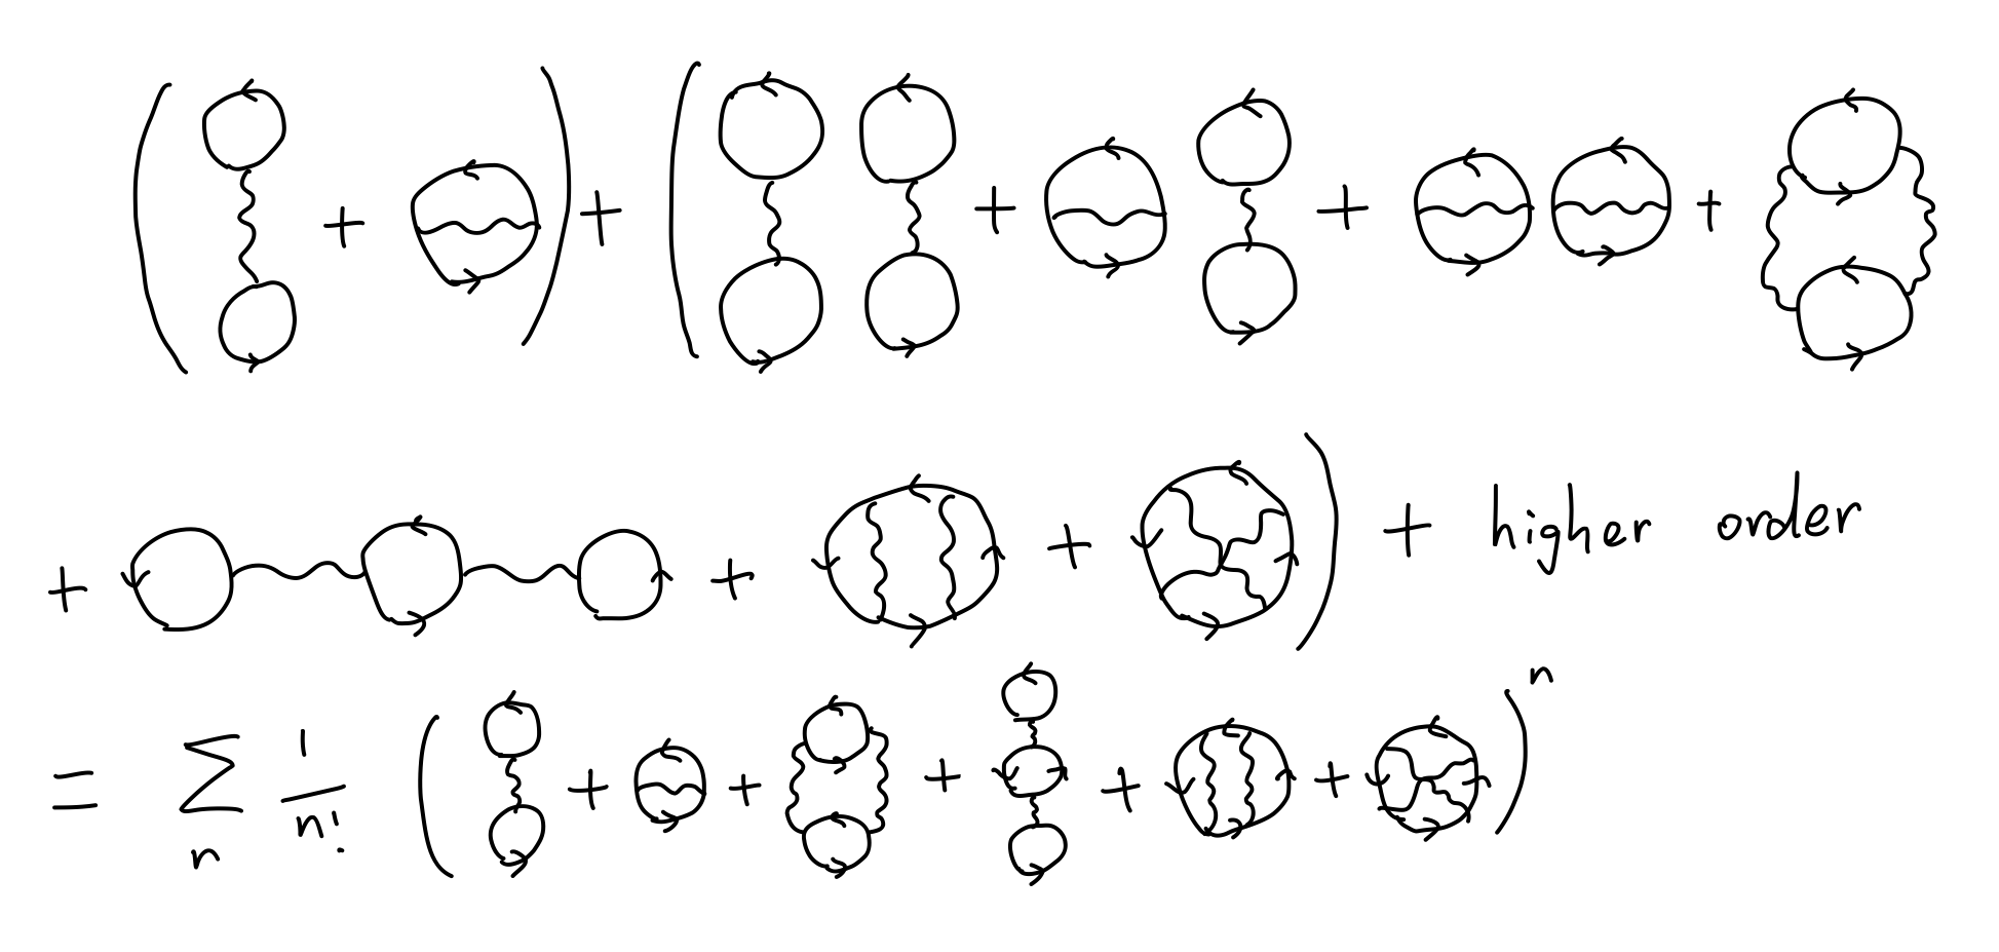
\includegraphics[height=6cm]{include/cluster}
\par\end{centering}
\caption{Cluster decomposition}
\end{figure}

\begin{eqnarray*}
\mathcal{Z} & = & \mathcal{Z}_{0}\sum_{n=0}^{\infty}\frac{\left(-1\right)^{n}}{n!}\left\langle S_{1}^{n}\right\rangle _{0}\\
 & = & \mathcal{Z}_{0}\prod_{n=0}^{\infty}\frac{1}{n!}\left(\sum_{m=1}^{\infty}\frac{\left(-1\right)^{m}}{m!}\left\langle S_{1}^{m}\right\rangle _{0}^{c}\right)^{n}\\
 & = & \mathcal{Z}_{0}\exp\left(\sum_{m=1}^{\infty}\frac{\left(-1\right)^{m}}{m!}\left\langle S_{1}^{m}\right\rangle _{0}^{c}\right).
\end{eqnarray*}
The perturbative expansion of free energy is then:
\[
\mathcal{F}=\mathcal{F}^{\left(0\right)}-T\sum_{m=1}^{\infty}\frac{\left(-1\right)^{m}}{m!}\left\langle S_{1}^{m}\right\rangle _{0}^{c}.
\]


\subsection{First order}

To the first order:

\begin{figure}[H]
\centering{}%
\begin{minipage}[t]{0.45\columnwidth}%
\subfloat[Hatree term.]{\begin{centering}
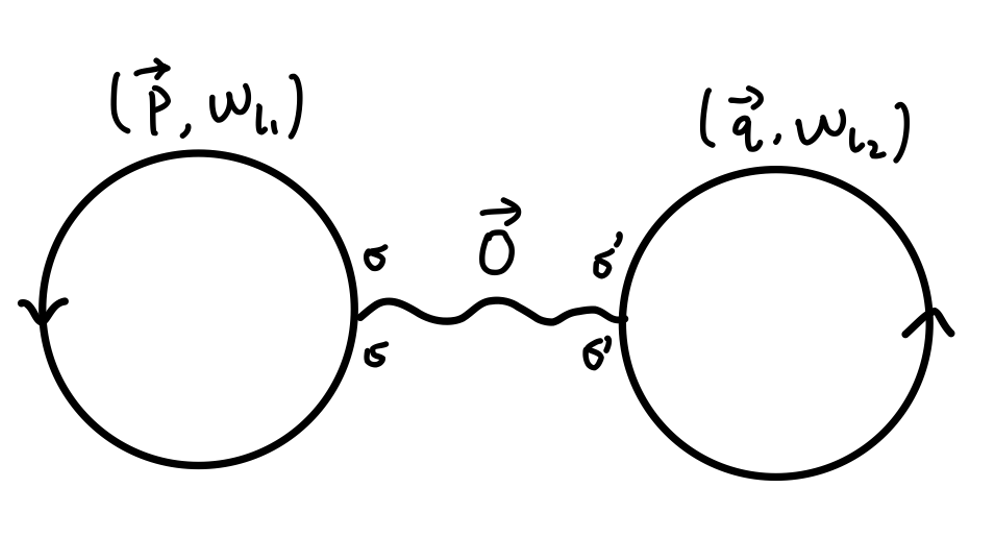
\includegraphics[height=4cm]{include/hartree}
\par\end{centering}

}%
\end{minipage}%
\begin{minipage}[t]{0.45\columnwidth}%
\subfloat[Fock term.]{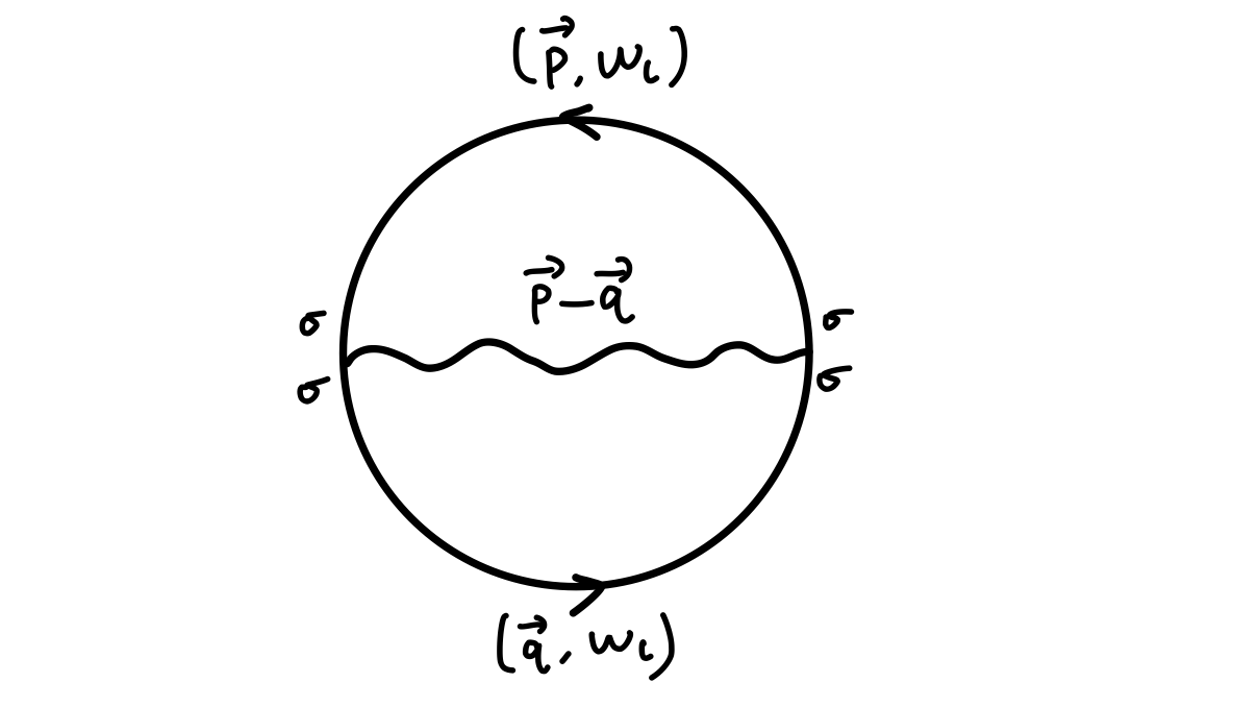
\includegraphics[height=4cm]{include/fock}

}%
\end{minipage}
\end{figure}

\begin{eqnarray*}
\mathcal{F}^{\left(1\right)} & = & \frac{T^{2}}{2L^{3}}\sum_{p_{1},p_{2},k}\sum_{\sigma,\sigma'}\left\langle \bar{\psi}_{p_{1}+k}^{\sigma}\bar{\psi}_{p_{2}-k}^{\sigma'}V\left(\bm{k}\right)\psi_{p_{2}}^{\sigma'}\psi_{p_{1}}^{\sigma}\right\rangle _{0}^{c}\\
 & = & \mathcal{F}_{Hatree}^{\left(1\right)}+\mathcal{F}_{Fock}^{\left(1\right)},
\end{eqnarray*}
where the Hartree and Fock term is:
\begin{eqnarray*}
\mathcal{F}_{Hatree}^{\left(1\right)} & = & \frac{2T^{2}}{L^{3}}\sum_{p_{1},p_{2}}G_{p_{1}}^{\left(0\right)}G_{p_{2}}^{\left(0\right)}V\left(\bm{0}\right)\\
 & = & 0,
\end{eqnarray*}
\begin{eqnarray*}
\mathcal{F}_{Fock}^{\left(1\right)} & = & -\frac{T^{2}}{L^{3}}\sum_{p_{1},p_{2}}G_{p_{2}}^{\left(0\right)}G_{p_{1}}^{\left(0\right)}V\left(\bm{p}_{1}-\bm{p}_{2}\right)\\
 & = & -\frac{1}{L^{3}}\sum_{\bm{p}_{1},\bm{p}_{2}}n_{F}\left(\epsilon_{\bm{p}_{1}}-\mu\right)n_{F}\left(\epsilon_{\bm{p}_{2}}-\mu\right)\frac{4\pi e^{2}}{\left|\bm{p}_{1}-\bm{p}_{2}\right|^{2}}\\
 & = & -L^{3}\int\frac{d^{3}p_{1}}{\left(2\pi\right)^{3}}\int\frac{d^{3}p_{2}}{\left(2\pi\right)^{3}}n_{F}\left(\epsilon_{\bm{p}_{1}}-\mu\right)n_{F}\left(\epsilon_{\bm{p}_{2}}-\mu\right)\frac{4\pi e^{2}}{\left|\bm{p}_{1}-\bm{p}_{2}\right|^{2}}.
\end{eqnarray*}
In low-T limit:

\[
\mathcal{F}_{Fock}^{\left(1\right)}\approx-\frac{2e^{2}L^{3}}{\left(2\pi\right)^{5}}\int_{p,q<k_{F}}\frac{d^{3}pd^{3}q}{\left|\bm{p}-\bm{q}\right|^{2}}.
\]
The integral is:

\begin{eqnarray*}
I & = & \int_{p,q<k_{F}}d^{3}\bm{p}d^{3}\bm{q}\frac{1}{\left|\bm{p}-\bm{q}\right|^{2}}\\
 & = & 4\pi\int_{0}^{k_{F}}p^{2}dp\int_{0}^{k_{F}}q^{2}dq\int_{-1}^{+1}d\left(\cos\theta\right)\int_{0}^{2\pi}d\theta\frac{1}{p^{2}+q^{2}-2pq\cos\theta}\\
 & = & 8\pi^{2}\int_{0}^{k_{F}}p^{2}dp\int_{0}^{k_{F}}q^{2}dq\int_{-1}^{+1}\frac{d\left(p^{2}+q^{2}-2pq\cos\theta\right)}{-2pq}\frac{1}{p^{2}+q^{2}-2pq\cos\theta}\\
 & = & 8\pi^{2}\int_{0}^{k_{F}}p^{2}dp\int_{0}^{k_{F}}q^{2}dq\frac{1}{pq}\ln\left|\frac{p+q}{p-q}\right|\\
 & = & 16\pi^{2}\int_{0}^{k_{F}}p^{3}dp\int_{0}^{1}dt\left[t\ln\left(\frac{1+t}{1-t}\right)\right]\\
 & = & 16\pi^{2}\int_{0}^{k_{F}}p^{3}dp\left[\int_{0}^{1}dx\left(x-1\right)\ln x+\int_{1}^{2}dx\left(x-1\right)\ln x\right]\\
 & = & 16\pi^{2}\int_{0}^{k_{F}}p^{3}dp\left.\left[\frac{t^{2}\ln t}{2}-\frac{t^{2}}{4}+t-t\ln t\right]\right|_{0}^{2}\\
 & = & 16\pi^{2}\int_{0}^{k_{F}}p^{3}dp\\
 & = & \left(2\pi\right)^{2}k_{F}^{4}.
\end{eqnarray*}
So the free energy to the first order is:

\[
\mathcal{F}^{\left(1\right)}=\mathcal{F}_{Fock}^{\left(1\right)}=-\frac{2e^{2}L^{3}k_{F}^{4}}{\left(2\pi\right)^{3}}.
\]


\subsection{Random phase approximation}

The largest perturbative contribution is the ring graphs:

\begin{figure}[H]
\begin{centering}
\includegraphics[angle=90,height=4cm]{\string"include/ring graph\string".png}
\par\end{centering}
\centering{}\caption{Ring graph}
\end{figure}

\[
F_{RPA}^{\left(n\right)}=-\frac{T}{2n}\sum_{q}\left(\frac{2T}{L^{3}}\sum_{p}G_{p}^{\left(0\right)}G_{p+q}^{\left(0\right)}\right)^{n},
\]
where $2n$ is the symmetry factor. To evaluate the $n^{th}$ order
free energy, we first calculate the polarization operator:

\begin{eqnarray*}
\Pi_{q} & \coloneqq & \frac{2T}{L^{3}}\sum_{\bm{p}}\sum_{\omega_{p}}G_{p}^{\left(0\right)}G_{p+q}^{\left(0\right)}\\
 & = & \frac{2T}{L^{3}}\sum_{\bm{p}}\sum_{\omega_{p}}\frac{1}{i\omega_{p}-\epsilon_{\bm{p}}+\mu}\cdot\frac{1}{i\left(\omega_{p}+\omega_{q}\right)-\epsilon_{\bm{p}+\bm{q}}+\mu}\\
 & = & \frac{2}{L^{3}}\sum_{\bm{p}}\frac{n_{F}\left(\epsilon_{\bm{p}+\bm{q}}-\mu\right)-n_{F}\left(\epsilon_{\bm{p}}-\mu\right)}{-i\omega_{q}+\epsilon_{\bm{p}+\bm{q}}-\epsilon_{\bm{p}}}\\
 & = & \frac{2}{\left(2\pi\right)^{3}}\int d^{3}p\frac{n_{F}\left(\epsilon_{\bm{p}+\bm{q}}-\mu\right)-n_{F}\left(\epsilon_{\bm{p}}-\mu\right)}{-i\omega_{q}+\epsilon_{\bm{p}+\bm{q}}-\epsilon_{\bm{p}}}.
\end{eqnarray*}
To evaluate the integration, first note that for small $\bm{q}$ and
low temperature, we can linearize the energy and distribution difference: 

\begin{eqnarray*}
\epsilon_{\bm{p}+\bm{q}}-\epsilon_{\bm{p}} & \approx & \frac{\bm{p}\cdot\bm{q}}{m},\\
n_{F}\left(\epsilon_{\bm{p}+\bm{q}}-\mu\right)-n_{F}\left(\epsilon_{\bm{p}}-\mu\right) & \approx & \frac{\partial n_{F}}{\partial\epsilon}\left(\epsilon_{\bm{p}}-\mu\right)\cdot\frac{\bm{p}\cdot\bm{q}}{m}\\
 & \approx & -\delta^{\left(3\right)}\left(\epsilon_{\bm{p}}-\mu\right)\cdot\frac{\bm{p}\cdot\bm{q}}{m}.
\end{eqnarray*}
So the integration becomes:

\begin{eqnarray*}
\Pi_{q} & \approx & \frac{-2}{\left(2\pi\right)^{3}}\int p_{F}^{2}dp\delta\left(\frac{p^{2}}{2m}-\mu\right)\int_{-1}^{+1}d\left(\cos\theta\right)\int_{0}^{2\pi}d\phi\frac{p_{F}q\cos\theta/m}{-i\omega_{q}+p_{F}q\cos\theta/m}\\
 & = & -\frac{1}{2\pi^{2}}\int p_{F}^{2}dp\delta\left(\frac{p^{2}}{2m}-\mu\right)\int_{-1}^{+1}d\left(\cos\theta\right)\frac{v_{F}q\cos\theta}{-i\omega_{q}+v_{F}q\cos\theta}\\
 & = & -\frac{1}{2\pi^{2}}\int p_{F}^{2}dp\delta\left(\frac{p^{2}}{2m}-\mu\right)\left[1+\frac{i\omega_{q}}{2v_{F}q}\ln\left(\frac{i\omega_{q}+v_{F}q}{i\omega_{q}-v_{F}q}\right)\right]\\
 & = & -\frac{mp_{F}}{\pi^{2}}\left[1-\frac{i\omega_{q}}{2v_{F}q}\ln\left(\frac{i\omega_{q}+v_{F}q}{i\omega_{q}-v_{F}q}\right)\right].
\end{eqnarray*}
where we have used

\[
\delta\left(f\left(z\right)\right)=\sum_{z_{k}}\frac{\delta\left(z-z_{k}\right)}{\left|f'\left(z_{k}\right)\right|}.
\]


\section{Self energy}

\begin{figure}[H]
\begin{centering}
\includegraphics[width=10cm]{\string"include/photon self energy\string".png}
\par\end{centering}
\centering{}\caption{Photon self energy}
\end{figure}

\begin{eqnarray*}
V_{eff}\left(q\right) & = & V\left(\bm{q}\right)+V\left(\bm{q}\right)\Pi_{q}V_{eff}\left(q\right)\\
 & = & \frac{V\left(\bm{q}\right)}{1-V\left(\bm{q}\right)\Pi_{q}}\\
 & \eqqcolon & \frac{V\left(\bm{q}\right)}{\epsilon\left(q\right)},
\end{eqnarray*}
where we have defined a dielectric function:

\[
\epsilon\left(q\right)\coloneqq1-V\left(\bm{q}\right)\Pi_{q}.
\]
For small $\bm{q}$ and $\omega_{q}$ :
\[
\omega_{q}\ll qv_{F},
\]

\[
\Pi\left(\bm{q},\omega_{q}\right)\approx-\frac{mp_{F}}{\pi^{2}}\eqqcolon-\nu_{0}.
\]
In this limit:
\[
V\left(q\right)\approx\frac{1}{V^{-1}\left(\bm{q}\right)+\nu_{0}}=\frac{4\pi e^{2}}{q^{2}+4\pi e^{2}\nu_{0}}\eqqcolon\frac{4\pi e^{2}}{q^{2}+\lambda^{-2}}.
\]
The $\lambda\coloneqq\left(4\pi e^{2}\nu_{0}\right)^{-1/2}$ is the
Thomas-Fermi screening length. To see the physical meaning, do the
inverse Fourier transformation:

\begin{eqnarray*}
V\left(r\right) & = & \int\frac{d^{3}q}{\left(2\pi\right)^{3}}e^{i\bm{q}\cdot r}\frac{4\pi e^{2}}{q^{2}+\lambda^{-2}}\\
 & = & \frac{e^{2}}{\pi}\int_{0}^{+\infty}q^{2}dq\int_{-1}^{+1}d\left(\cos\theta\right)\frac{e^{iqr\cos\theta}}{q^{2}+\lambda^{-2}}\\
 & = & \frac{e^{2}}{i\pi r}\int_{0}^{+\infty}dq\frac{q}{q^{2}+\lambda^{-2}}\left(e^{+iqr}-e^{-iqr}\right)\\
 & = & \frac{e^{2}}{i\pi r}\int_{-\infty}^{+\infty}dq\frac{q}{q^{2}+\lambda^{-2}}e^{+iqr}.
\end{eqnarray*}

\begin{figure}[H]
\begin{centering}
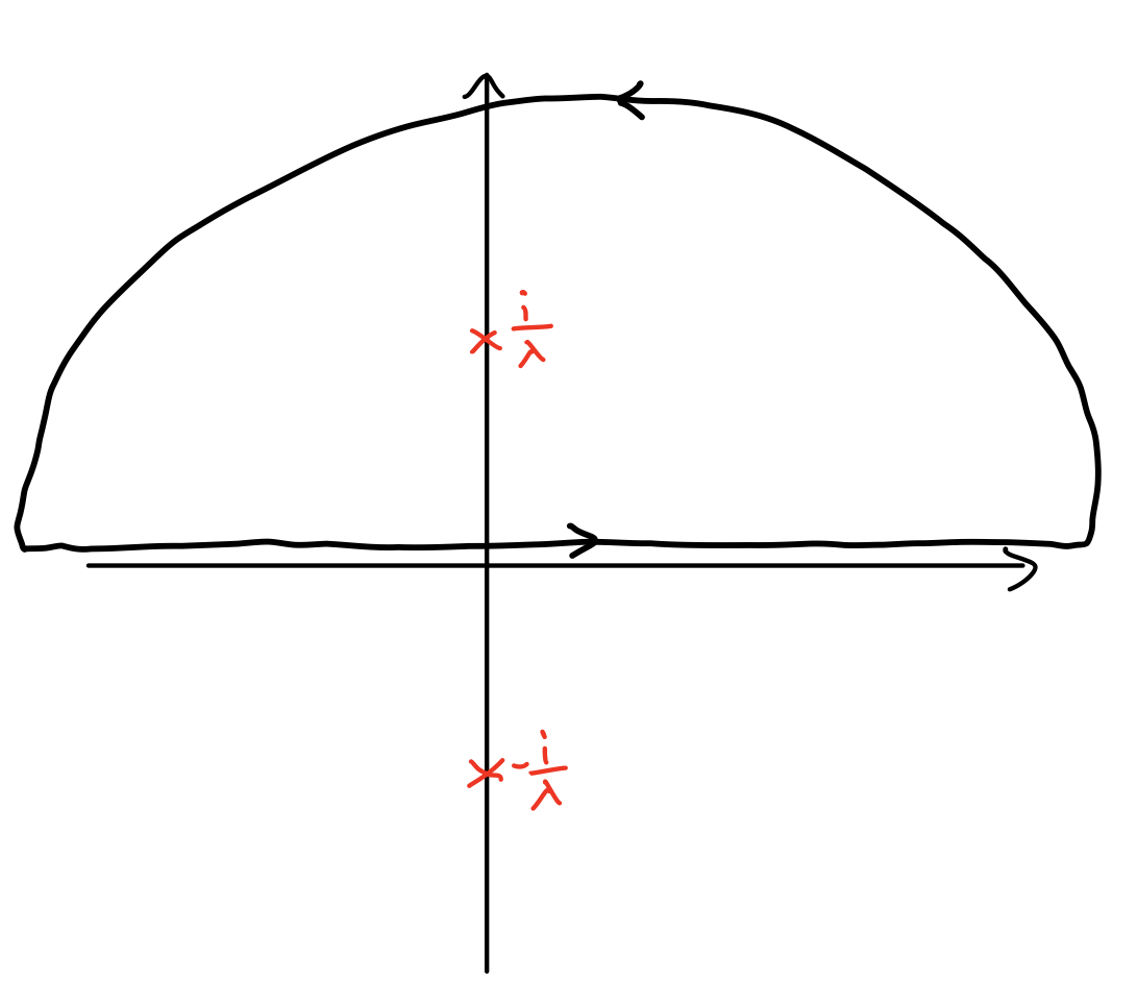
\includegraphics[height=6cm]{include/contour1}
\par\end{centering}
\centering{}\caption{Integration contour}
\end{figure}

Apply residue theorem to get the result:

\[
\left.Res\left[\frac{q}{q^{2}+\lambda^{-2}}e^{+iqr}\right]\right|_{q=\frac{i}{\lambda}}=\frac{1}{2}e^{-\frac{r}{\lambda}},
\]

\[
V\left(r\right)=\frac{e^{2}}{r}e^{-\frac{r}{\lambda}}.
\]

\end{document}
